\documentclass[../../../analisi-dei-requisiti.tex]{subfiles}
% \documentclass[components/casi-duso-app]{subfiles}

\begin{document}

\subsubsection{UUC1: Registrazione}%
\label{subs:UUC1}

\begin{figure}[H]
  \centering
  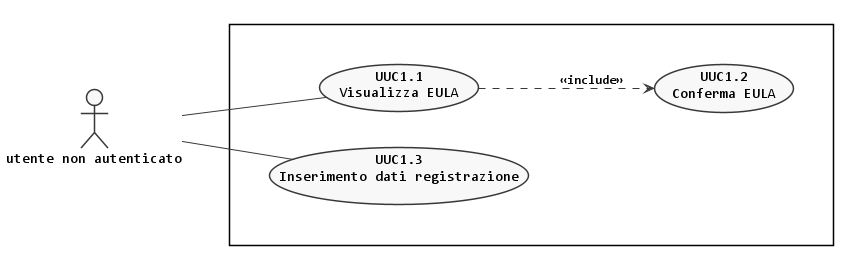
\includegraphics[width=150mm]{registrazione.png}
  \caption{UUC1: Registrazione}%
  \label{fig:uuc1}
\end{figure}

\begin{description}
  \item[Caso d’uso:] UUC1;
  \item[Titolo:] Registrazione;
  \item[Attori primari:] utente non autenticato;
  \item[Precondizione:] l'utente non è registrato al servizio;
  \item[Postcondizione:] la registrazione va a buon fine e l'utente è registrato;
  \item[Scenario principale:]
        \begin{enumerate}
          \item prima di procedere con la registrazione, l'utente visualizza il \glossario{EULA} e per continuare deve accettare i vincoli stabiliti da essa;
          \item una volta accettato il EULA, l'utente provvede all'inserimento dei dati personali per la registrazione.
        \end{enumerate}
\end{description}


\subsubsection{UUC1.1: Visualizza EULA}%
\label{subs:UUC1.1}
\begin{description}
  \item[Caso d’uso:] UUC1.1;
  \item[Titolo:] Visualizza EULA\@;
  \item[Attori primari:] utente non autenticato;
  \item[Precondizione:] l'utente è all'interno della schermata di registrazione;
  \item[Postcondizione:] l'utente prima della sua registrazione deve poter visualizzare il EULA\@;
  \item[Scenario principale:]
        \begin{enumerate}
          \item l'utente visualizza una schermata con tutti i vincoli da accettare presenti nel EULA\@.
        \end{enumerate}
\end{description}

\subsubsection{UUC1.2: Conferma EULA}%
\label{subs:UUC1.2}
\begin{description}
  \item[Caso d’uso:] UUC1.2;
  \item[Titolo:] Conferma EULA\@;
  \item[Attori primari:] utente non autenticato;
  \item[Precondizione:] l'utente è all'interno della schermata di registrazione;
  \item[Postcondizione:] l'utente continua la registrazione in quanto ha accettato il EULA\@;
  \item[Scenario principale:]
        \begin{enumerate}
          \item è presente un'opzione per accettare il EULA\@: in caso affermativo, si può continuare con la registrazione.
        \end{enumerate}
\end{description}

\subsubsection{UUC1.3: Inserimento dati registrazione}%
\label{subs:UUC1.3}

\begin{figure}[H]
  \centering
  \scalegraphics{inserimento-dati-registrazione.png}
  \caption{UUC1.3: Inserimento dati registrazione}%
  \label{fig:uuc1_3}
\end{figure}

\begin{description}
  \item[Caso d’uso:] UUC1.3;
  \item[Titolo:] Inserimento dati registrazione;
  \item[Attori primari:] utente non autenticato;
  \item[Precondizione:] il sistema deve rendere disponibile la pagina di registrazione;
  \item[Postcondizione:] l'utente ha inserito correttamente tutti i dati necessari alla registrazione;
  \item[Scenario principale:]
        \begin{enumerate}
          \item l'utente compila tutti i dati necessari alla registrazione.
        \end{enumerate}
  \item[Estensioni:]
        \begin{enumerate}
          \item se la mail inserita non è valida, l'utente visualizzerà un errore~\ref{subs:UUC1.3.5};
          \item se la password inserita non è valida, l'utente visualizzerà un errore~\ref{subs:UUC1.3.6};
          \item se la conferma della password inserita non è valida, l'utente visualizzerà un errore~\ref{subs:UUC1.3.7};
          \item se non vengono inseriti tutti i dati anagrafici, l'utente visualizzerà un errore~\ref{subs:UUC1..8}.
        \end{enumerate}
\end{description}



\subsubsection{UUC1.3.1: Registrazione email}%
\label{subs:UUC1.3.1}
\begin{description}
  \item[Caso d’uso:] UUC1.3.1;
  \item[Titolo:] Registrazione email;
  \item[Attori primari:] utente non autenticato;
  \item[Precondizione:] il sistema deve rendere disponibile la possibilità di inserire la email per la registrazione;
  \item[Postcondizione:] l'utente ha inserito la email in modo corretto;
  \item[Scenario principale:]
        \begin{enumerate}
          \item l'utente inserisce la propria email.
        \end{enumerate}
  \item[Estensioni:]
        \begin{enumerate}
          \item se la mail è scritta in una forma non corretta, verrà visualizzato un errore di email non valida~\ref{subs:UUC1.3.5}.
        \end{enumerate}
\end{description}



\subsubsection{UUC1.3.2: Registrazione password}%
\label{subs:UUC1.3.2}
\begin{description}
  \item[Caso d’uso:] UUC1.3.2;
  \item[Titolo:] Registrazione password;
  \item[Attori primari:] utente non autenticato;
  \item[Precondizione:] il sistema deve rendere disponibile la possibilità di inserire la password per la registrazione;
  \item[Postcondizione:] l'utente ha inserito la password in modo corretto;
  \item[Scenario principale:]
        \begin{enumerate}
          \item l'utente inserisce la propria password.
        \end{enumerate}
  \item[Estensioni:]
        \begin{enumerate}
          \item se la password non rispetta determinati vincoli, verrà visualizzato un errore di password non valida~\ref{subs:UUC1.3.6}.
        \end{enumerate}
\end{description}



\subsubsection{UUC1.3.3: Conferma password}%
\label{subs:UUC1.3.3}
\begin{description}
  \item[Caso d’uso:] UUC1.3.3;
  \item[Titolo:] Conferma password;
  \item[Attori primari:] utente non autenticato;
  \item[Precondizione:] il sistema deve rendere disponibile la possibilità di inserire la password nuovamente per una conferma;
  \item[Postcondizione:] l'utente ha inserito la conferma della password in modo corretto;
  \item[Scenario principale:]
        \begin{enumerate}
          \item l'utente inserisce la password nuovamente per la conferma.
        \end{enumerate}
  \item[Estensioni:]
        \begin{enumerate}
          \item se la password inserita non è uguale a quella precedente, verrà visualizzato un errore di conferma password non valida~\ref{subs:UUC1.3.7}.
        \end{enumerate}
\end{description}



\subsubsection{UUC1.3.4: Inserimento dati anagrafici}%
\label{subs:UUC1.3.4}
\begin{description}
  \item[Caso d’uso:] UUC1.3.4;
  \item[Titolo:] Inserimento dati anagrafici;
  \item[Attori primari:] utente non autenticato;
  \item[Precondizione:] il sistema deve rendere disponibile la schermata di registrazione riguardante i dati anagrafici;
  \item[Postcondizione:] l'utente ha inserito i dati anagrafici in modo corretto;
  \item[Scenario principale:]
        \begin{enumerate}
          \item l'utente inserisce i propri dati anagrafici.
        \end{enumerate}
  \item[Estensioni:]
        \begin{enumerate}
          \item se uno o più dati anagrafici inseriti non rispettano determinati vincoli, verrà visualizzato un errore~\ref{subs:UUC1.3.8}.
        \end{enumerate}
\end{description}

\subsubsection{UUC1.3.5: Mail registrazione non valida}%
\label{subs:UUC1.3.5}
\begin{description}
  \item[Caso d’uso:] UUC1.3.5;
  \item[Titolo:] Mail registrazione non valida;
  \item[Attori primari:] utente non autenticato;
  \item[Precondizione:] l'utente non inserisce la mail in modo corretto;
  \item[Postcondizione:] l'applicazione mobile comunica all'utente l'errore;
  \item[Scenario Principale:]
        \begin{enumerate}
          \item l'utente visualizza il messaggio d'errore, in quanto la mail inserita non è scritta correttamente.
        \end{enumerate}
\end{description}

\subsubsection{UUC1.3.6: Password registrazione non valida}%
\label{subs:UUC1.3.6}
\begin{description}
  \item[Caso d’uso:] UUC1.3.6;
  \item[Titolo:] Password registrazione non valida;
  \item[Attori primari:] utente non autenticato;
  \item[Precondizione:] l'utente non rispetta i vincoli imposti per la creazione della password;
  \item[Postcondizione:] l'applicazione mobile comunica all'utente l'errore;
  \item[Scenario Principale:]
        \begin{enumerate}
          \item l'utente visualizza il messaggio d'errore, in quanto la password inserita non rispetta i vincoli del sistema.
        \end{enumerate}
\end{description}

\subsubsection{UUC1.3.7: Conferma password registrazione non valida}%
\label{subs:UUC1.3.7}
\begin{description}
  \item[Caso d’uso:] UUC1.3.7;
  \item[Titolo:] Conferma password registrazione non valida;
  \item[Attori primari:] utente non autenticato;
  \item[Precondizione:] l'utente non inserisce correttamente la stessa password inserita nel campo precedente;
  \item[Postcondizione:] l'applicazione mobile comunica all'utente l'errore;
  \item[Scenario Principale:]
        \begin{enumerate}
          \item l'utente visualizza il messaggio d'errore, in quanto la password e la sua conferma non corrispondono.
        \end{enumerate}
\end{description}

\subsubsection{UUC1.3.8: Dati anagrafici registrazione non validi}%
\label{subs:UUC1.3.8}
\begin{description}
  \item[Caso d’uso:] UUC1.3.8;
  \item[Titolo:] Dati anagrafici registrazione non validi;
  \item[Attori primari:] utente non autenticato;
  \item[Precondizione:] l'utente non inserisce tutti i campi che riguardano i dati anagrafici;
  \item[Postcondizione:] l'applicazione mobile comunica all'utente l'errore;
  \item[Scenario Principale:]
        \begin{enumerate}
          \item l'utente visualizza il messaggio d'errore, in quanto devono essere compilati tutti i campi dei dati anagrafici.
        \end{enumerate}
\end{description}

\end{document}
